% 
% Annual Cognitive Science Conference
% Sample LaTeX Paper -- Proceedings Format
% 

% Original : Ashwin Ram (ashwin@cc.gatech.edu)       04/01/1994
% Modified : Johanna Moore (jmoore@cs.pitt.edu)      03/17/1995
% Modified : David Noelle (noelle@ucsd.edu)          03/15/1996
% Modified : Pat Langley (langley@cs.stanford.edu)   01/26/1997
% Latex2e corrections by Ramin Charles Nakisa        01/28/1997 
% Modified : Tina Eliassi-Rad (eliassi@cs.wisc.edu)  01/31/1998
% Modified : Trisha Yannuzzi (trisha@ircs.upenn.edu) 12/28/1999 (in process)
% Modified : Mary Ellen Foster (M.E.Foster@ed.ac.uk) 12/11/2000
% Modified : Ken Forbus                              01/23/2004
% Modified : Eli M. Silk (esilk@pitt.edu)            05/24/2005
% Modified: Niels Taatgen (taatgen@cmu.edu) 10/24/2006

%% Change ``a4paper'' in the following line to ``letterpaper'' if you are
%% producing a letter-format document.

\documentclass[10pt,letterpaper]{article}

\usepackage{cogsci}
\usepackage{bbm,amsmath,amssymb}
\usepackage{pslatex}
\usepackage{natbib}
\usepackage{bm}
\usepackage[usenames,dvipsnames]{xcolor}
\usepackage{tikz}
\usetikzlibrary{arrows}
\usepackage{verbatim}
\newcommand{\tb}[1]{\textcolor{Blue}{#1}}
%\usepackage{apacite}


\title{A Resource-Rational Approach to the Frame Problem}
 %NDG: ...or something else?
 %TFI: What do you think of this, or some variation?
 
 
\author{{\large \bf Noah D. Goodman} (ngoodman@stanford.edu), {\large \bf Thomas F. Icard, III} (icard@stanford.edu) \\
  Departments of Psychology and Philosophy, Stanford University}
  %NDG: you can be first if you want, since you did the main writing. or we could do a ``contributed equally'' note.
  %TFI: Thanks. Either way is fine with me!

\begin{document}

\maketitle


\begin{abstract}
Blah blah.. \vspace{2.2in}

\textbf{Keywords:} 
frame problem, bounded-resource-rationality, causal reasoning, alternative neglect.
\end{abstract}

\section{Introduction}

To any inference or decision problem, there is no \emph{a priori} bound on what aspects of a person's knowledge may be usefully, or even critically, applied. In principle, anything could be related to anything. 
This challenge is sometimes referred to as the \emph{frame problem}, characterized by \cite{Glymour1987} as: ``Given an enormous amount of stuff, and some task to be done using some of the stuff, what is the \emph{relevant stuff} for the task?'' (65). The question is foundational to reasoning and rationality. 
Part of what makes people so smart is their ability to solve the frame problem, ignoring those aspects of the world (and their knowledge of it) that are irrelevant to the problem at hand, thereby simplifying the underlying reasoning task, turning an intractable problem into a tractable one.

Not all of the psychological literature paints a picture of human reasoners as so efficient, however. In the literature on causal reasoning, there is a robust empirical finding that subjects often neglect causal variables, including those that are in principle accessible to the subject, which would sometimes allow the subject to make better, more accurate inferences. So called \emph{alternative neglect} is an especially well documented phenomenon, in which subjects ignore alternative possible causes of some event (\citealt{Fischhoff1978,KlaymanHa,Fernbach2011}, \emph{inter alia}), even when doing so leads to incorrect inferences, and would evidently not require a significant  amount of additional effort. More generally, at least in the causal domain, subjects tend to consider ``smaller'' models of the world than would be relevant to the task at hand, given the subject's knowledge and reasoning abilities. This has led many to criticize the behavior as normatively objectionable. Perhaps people are ignoring too much of their knowledge.

We would like to suggest that alternative neglect and related phenomena may be natural consequences of a general mechanism for sifting the most pertinent information from all other knowledge---that is, for solving the frame problem with regard to causal knowledge. Assuming a person's causal knowledge can be represented (at least implicitly) in terms of a very large directed graphical model, the \emph{causal} frame problem arises because computations involving the entire model promise to be intractable. Somehow the mind must focus in on some ``submodel'' of the full model that suffices for the task at hand. In as far as a proper submodel may nonetheless neglect relevant causal information, this may lead to inaccuracy. The suggestion is that, perhaps the mind tolerates local and occasional inaccuracy in order to achieve a more global efficiency. 
%NDG: need to introduce the causal frame problem and the idea of a sub-model before here.
%TFI: How does this look?
To substantiate this claim, we need a better understanding of what it is for a submodel to be more or less apt for a task, from the perspective of a reasoner with bounded time and resources. It is clear that human reasoners cannot consult an indefinitely detailed mental model of the world for every inference task. So what kind of simpler model \emph{should} a reasoner consult for a given task?

This work follows a line of research in cognitive science concerned with \emph{bounded} or \emph{resource rationality} (\citealt{Simon1957,Gigerenzer1996}, \emph{inter alia}), and specifically in the context of probabilistic models, and approximations thereto \citep{Vul2014}. In addition to inherent interest, it has recently been suggested that considerations of bounded rationality may play a methodological role in sharpening the search for reasonable accounts of the cognitive processes underlying inductive inference \citep{Griffiths2014,Icard2014}. However, in this tradition there has been more of a focus on the algorithm used for inference in a given model, and less attention paid to questions of model selection.

In this paper we offer a framework for solving the causal frame problem by selecting rational submodels, provide several illustrative examples, and address some of the empirical findings concerning alternative neglect.

\section{Resource-Rational Submodels}

Let $P(\textbf{X})$ be a joint probability distribution over random variables $\textbf{X} = X_1,X_2,\dots$, and define a \emph{query} to be a partition $\langle \textbf{X}_q;\textbf{X}_l;\textbf{X}_e\rangle$ of \textbf{X} into \emph{query variables}, \emph{latent variables}, and \emph{evidence variables}, respectively. A typical query task is to find values of $\textbf{X}_q$ that maximize the conditional probability $P(\textbf{X}_q\mid \textbf{X}_e = \textbf{v})$, marginalizing over values of $\textbf{X}_l$. Clearly, the difficulty of this and related tasks scales with the number of variables. We will be interested in smaller models with fewer variables: a sublist $\textbf{X}^*$ of $\textbf{X}$ with associated distribution $P^*(\textbf{X}^*)$, and associated partition $\langle \textbf{X}_q;\textbf{X}_l^*;\textbf{X}_e^*\rangle$, so that only latent and evidence variables are ignored. The canonical way of choosing $P^*$ given $\textbf{X}^*$ is as to treat all neglected variables as though they are uniform, effectively ignoring any (direct or indirect) influence they may have on $\textbf{X}_q$.

%NDG: we should say something about why these two questions are of interest?
Given $P(\textbf{X})$ and $P^*(\textbf{X}^*)$, there are at least two kinds of questions we would like to ask:\footnote{Strictly speaking, the second can be seen a special case of the first, with a logarithmic scoring rule \citep{Bernardo}.} \begin{enumerate}
  \item Given a decision problem with action space $\mathcal{A}$ and utility function $U:\textbf{X}_q\times \mathcal{A} \rightarrow\mathbb{R}$, and assuming fixed a (stochastic) choice rule $\Psi_Q$ taking a distribution $Q$ over $\textbf{X}_q$ to a distribution on actions, what are the respective expected utilities of using $P$ and $P^*$ under (assumed ``true'') distribution $P$? That is, how great is the following difference $\Delta_{P,P^*}$? \end{enumerate}
  $$\Delta_{P,P^*} \;\; = \;\; \mathbb{E}_{\textbf{x}\sim P}\;\mathbb{E}_{A \sim \Psi_{P}}\;U(\textbf{x},A) \,-\, \mathbb{E}_{\textbf{x} \sim P}\;\mathbb{E}_{A \sim \Psi_{P^*}}\;U(\textbf{x},A)$$
  \begin{enumerate}
  \item[2.] How far is $P^*$ from $P$ in information distance, for the variables $\textbf{X}_q$ of interest? That is, what is the Kullback-Leibler divergence between $P$ and $P^*$ with respect to $\textbf{X}_q$?
\end{enumerate}$$KL(P \;||\; P^*)  =  \sum_{\textbf{x}} P(\textbf{X}_q = \textbf{x} \mid \textbf{X}_{e} = \textbf{v})\; \mbox{log} \; \frac{P(\textbf{X}_q = \textbf{x} \mid \textbf{X}_{e} = \textbf{v})}{P^*(\textbf{X}_q = \textbf{x} \mid \textbf{X}^*_{e} = \textbf{v}^*)}$$
The first of these captures how well an agent will fare by using the approximate submodel, as compared with the full model, holding fixed a procedure for using this model to choose an action. For instance, the agent might use this distribution to compute expected utility, or to \emph{sample} from the model in order to approximate expected utility (see, e.g,. \citealt{Vul2014}). The second question asks how far off the approximate model is from the ``true'' model in its probabilistic predictions. In general we will expect that $KL(P \;||\; P^*) > 0$, and $\mathbb{E}_{\textbf{x}\sim P}\;\mathbb{E}_{A \sim \Psi_{P}}\;U(\textbf{x},A) > \mathbb{E}_{\textbf{x} \sim P}\;\mathbb{E}_{A \sim \Psi_{P^*}}\;U(\textbf{x},A)$. However, in line with other work on resource rationality, assuming the requisite computations using distribution $P$ come with a greater cost than when using $P^*$, this difference in cost may well be worth the difference in accuracy or utility.

Suppose we have a cost function $c: \mathcal{P}\rightarrow\mathbb{R}^+$, assigning a real cost to each approximation $P^* \in \mathcal{P}$. For instance, $c$ may simply charge a constant amount for each variable used in the associated submodel. Given a set $\mathcal{P}$ of approximations, we can then ask for the \emph{resource-optimal} approximation  in either of the above two senses. For instance, with KL-divergence, of interest is the distribution $P^*$ that optimally trades off cost against KL-distance from the true distribution $P$: 

\begin{equation} \underset{P^*\in\mathcal{P}}{\textnormal{min}} \; KL(P\;||\;P^*) + c(P^*)\;.\label{optimal}\end{equation}


In what follows we illustrate these ideas with three examples using familiar graphical models. The first example, of an HMM, demonstrates an extreme case of the frame problem in which the initial model is potentially infinite. In this case we show that the resource optimal submodel is not only finite, but often quite small, and in many instances includes just a single node. The second example, of a causal Bayes net, shows that under a sampling scheme for decision making \citep{Vul2014}, the submodel actually outperforms the ``ideal'' full model in many cases, even without taking costs into account. Finally, the third example, also involving small Bayes nets, reveals that certain kinds of inferences may be subject to greater information loss resulting from alternative neglect than others. Recent empirical literature shows that people respect this difference, suggesting that there may indeed be an element of resource rationality in neglect behavior.

\section{Hidden Markov Models}

A Hidden Markov Model is given by a time-labeled sequence of state variables $X_1,X_2,\dots$, with transition probability $P(X_{t+1}\mid X_t)$, and a sequence of evidence variables $Y_1,Y_2,\dots$, with emission probabilities $P(Y_t\mid X_t)$. In a typical inference task, after observing some values of $Y$ (blue), we are interested in the value of $X_{t+1}$ (beige) at time $t+1$:

\begin{figure}[h] 
\begin{center}
  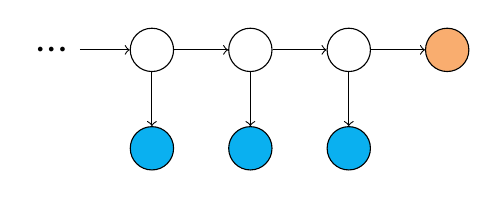
\begin{tikzpicture}
  
  
  \node (s0) at (-.25,1.25)  {$\textbf{\dots}$};
  
  \node (s1) at (1,1.25) [circle,draw=black,minimum size=0.55cm] {};

  \node (s2) at (1,0) [circle,draw=black,fill=ProcessBlue,minimum size=0.55cm] {};
  
  \node (s3) at (2.25,1.25) [circle,draw=black,minimum size=0.55cm] {};
  
  \node (s4) at (2.25,0)  [circle,draw=black,fill=ProcessBlue,minimum size=0.55cm] {};
  
  \node (s5) at (3.5,1.25) [circle,draw=black,minimum size=0.55cm] {};
  
  \node (s6) at (3.5,0)  [circle,draw=black,fill=ProcessBlue,minimum size=0.55cm] {};
  
  \node (s7) at (4.75,1.25) [circle,draw=black,minimum size=0.55cm,fill=Apricot] {};
 
  \path (s0) edge[->] (s1);
  
  \path (s1) edge[->] (s2);
  
  \path (s1) edge[->] (s3);
  
  \path (s3) edge[->] (s4);
  
  \path (s3) edge[->] (s5);
  
  \path (s5) edge[->] (s6);
  
  \path (s5) edge[->] (s7);
  
 \end{tikzpicture}
\end{center} 
\end{figure} 
\noindent For instance, variables $X$ might be whether there is high or low air pressure, while observations $Y$ are of sun or clouds. While in principle determining $X_{t+1}$---what the weather will be like tomorrow---could depend on indefinitely earlier observations and states---indeed, the model could even be infinite---one has the intuition that ``looking back'' only a few steps should be sufficient for typical purposes.

For a first illustration, consider a simple HMM with binary variables $X_t$ and $Y_t$, and probabilities as follows:
$$P(X_{t+1}=1\mid X_t=1) = P(X_{t+1}=0\mid X_t=0) = 0.9$$
$$P(Y_{t}=1\mid X_t=1) = P(Y_{t}=0\mid X_t=0) = 0.8$$
Our class $\mathcal{P}$ of approximate distributions includes all truncations of the model at variable $X_{t-N}$, in which case we assume the distribution $P^{*}(X_{t-N})$ is uniform. In Figure \ref{hmm}1 is a graph showing the KL-distance between the full model and a submodel with only $N$ previous time steps included.
%NDG: we need to say what this particular HMM is (two states, what transitions). also maybe give a sense of the KL curve as a function of the ``stiffness'' (second eigenvalue?)  of the transition function. plot stiffness vs optimal truncation depth?
% This is my best attempt at that. Look reasonable?

 \begin{figure}[h]  \begin{center}
\includegraphics[scale=0.3]{hmm1.pdf} \caption{Dropoff in KL as function of number of nodes.} \end{center} 
\label{hmm}\end{figure} 
We chose this particular model for illustration because the KL-distance is relatively high for the submodel with only one node. Nonetheless, even for this model, the value drops off rather dramatically with only a few additional nodes. This model has a low mixing rate, as measured by the second eigenvalue ($\lambda_2$) of the transition matrix for the underlying Markov model (the transition probabilities). In general, a higher $\lambda_2$ value means a lower mixing rate. One might expect that in such cases it is more detrimental to ignore previous state variables. If we look at the graph of KL-distances as a function of $\lambda_2$, holding fixed the observation probabilities as above, we see that this model (for which $\lambda_2 = 0.8$) is indeed near the higher end:

 \begin{figure}[h]  \begin{center}
\includegraphics[scale=0.33]{kl-eigenvalue-5.pdf} \caption{KL-distance for an approximate model with only one state variable, as a function of second eigenvalue $\lambda_2$.} \end{center} 
\label{kl-eigen}\end{figure}

If we now factor in the cost of including more nodes in the approximate HMM, we can determine for different values of $\lambda_2$, and for different assumptions about cost of a node, what the optimal number of nodes to include will be, in line with the expression (\ref{optimal}) above. In the following graph we assume the cost of an additional node is $0.02$.

 \begin{figure}[h]  \begin{center}
\includegraphics[scale=0.33]{kl-eigenvalue-6.pdf} \caption{Optimal number of nodes, given a cost of $0.02$ per node, as a function of second eigenvalue $\lambda_2$.} \end{center} 
\label{kl-eigen1}\end{figure}

\noindent For relatively low values of $\lambda_2$, it is not worth the cost to include more than a single state variable in the model. This is perhaps not surprising, given the low KL-values in Fig. \ref{kl-eigen}2. However, even in models with significantly higher KL-distances in general, it does not pay to include more than one or two additional nodes. Note in particular that, while a model with $\lambda_2=0.8$ is further from the true model than one with $\lambda_2=0.7$, only in the latter case does the marginal difference in KL-value between including two and three nodes merit the cost of including the third node. 

As Fig. \ref{kl-eigen1}3 indicates, the optimal number of nodes to include in an HMM is not only finite, but typically quite small.

\section{Neglecting Alternative Causes}

Consider next a simple causal model under a Noisy-Or parameterization \citep{Cheng}. That is, suppose we have binary causal variables $\textbf{X}$, taking on values 0 or 1, and conditional probabilities given in terms of weights $\theta_{Y,X}$ codifying the influence of parent $Y$ on a variable $X$, and a ``background bias'' parameter $\beta$: $$P\big(X\mid \textbf{pa}(X)\big) \quad = \quad 1-\Big((1-\beta)\prod_{Y \in \textbf{pa}(X)} (1-\theta_{Y,X})^Y\Big)$$
This model has the convenient property that, deleting nodes from the graph still leaves us with a well-defined distribution.

Suppose in particular we have variables $A,B,C,D$ with weights $\theta_1, \theta_2$, and $\theta_3$, as depicted on the left in Figure \ref{noisy-or}.
\begin{figure}[h] 
\begin{center}
  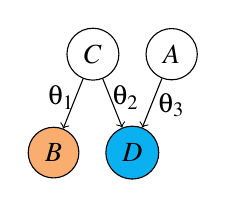
\begin{tikzpicture}
  
  \node (s0) at (.5,1.25) [circle,draw=black] {$C$};
  
  \node (s1) at (1.5,1.25) [circle,draw=black] {$A$};
  
  \node (s2) at (0,0) [circle,draw=black,fill=Apricot] {$B$};
  
  \node (s3) at (1,0) [circle,draw=black,fill=ProcessBlue] {$D$};
 
  \path (s0) edge[->] (s2);
  
  \path (s0) edge[->] (s3);
  
  \path (s1) edge[->] (s3);
  
  \node (i1) at (.1,.7) {$\theta_1$};
  
  \node (i1) at (.92,.7) {$\theta_2$};
  
  \node (i1) at (1.5,.6) {$\theta_3$};
  
 \end{tikzpicture} \hspace{0.7in}
   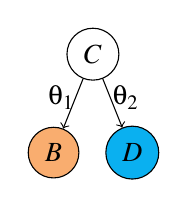
\begin{tikzpicture}
  
  \node (s0) at (.5,1.25) [circle,draw=black] {$C$};
  
  \node (s2) at (0,0) [circle,draw=black,fill=Apricot] {$B$};
  
  \node (s3) at (1,0) [circle,draw=black,fill=ProcessBlue] {$D$};
 
  \path (s0) edge[->] (s2);
  
  \path (s0) edge[->] (s3);
  
  \node (i1) at (.1,.7) {$\theta_1$};
  
  \node (i1) at (.92,.7) {$\theta_2$};
  
 \end{tikzpicture}
\end{center} \caption{Full Model versus Partial Submodel} \label{noisy-or}
\end{figure} 

\noindent Imagine, for instance, a case of social reasoning, in which: \begin{itemize} \item[] $A$: ``Mary has lost her usual gloves'' \item[] $B$: ``Mary has her bicycle with her''  \item[] $C$: ``Mary is going cycling"  \item[] $D$:  ``Mary is wearing cycling gloves'' \end{itemize}
Observing that Mary is wearing cycling gloves makes it more likely that she is going cycling, and therefore that she has her bike with her. But this is attenuated by the alternative possible cause, that she lost her other gloves. Our question in this case is, how much worse will a reasoner fare by ignoring alternative cause $A$, that is, by using the smaller submodel  in Figure \ref{noisy-or}, on the right?

To assess this question, we can look at both the difference in expected utility and the KL-divergence between using the ``true'' distribution $P$ and the approximate distribution $P^*$, for $B$ given $D=1$. Table \ref{table1} below presents example KL-values for different settings of model parameters (here and throughout this subsection, we set $\beta = 0.05$).

\begin{table}[h]  \begin{center}
\begin{tabular}{c | c | c | c | c || c}
 $P(C)$ & $P(A)$ & $\theta_1$ & $\theta_2$ & $\theta_3$ & $KL(P \;\vert\vert\; P^*)$ \\ \hline
 $0.5$ & $0.5$ & $1$ & $1$ & $1$  & $0.594$ \\
  $0.5$ & $0.5$ & $1$ & $0.5$ & $0.9$  & $0.467$ \\
  $0.5$ & $0.5$ &$1$ & $0.5$ & $0.5$  & $0.270$ \\
 $0.5$ & $0.5$ & $1$ & $0.9$ & $0.5$  & $0.261$ \\
  $0.3$ & $0.1$ & $1$ & $1$ & $1$ & $0.121$ \\
 $0.5$ & $0.5$ &  $0.9$ & $0.1$ & $0.5$  & $0.081$ \\
  $0.3$ & $0.1$ & $0.9$ & $0.1$ & $0.5$ & $0.023$ \\
 $0.5$ & $0.5$ & $0.1$ & $0.1$ & $0.1$ & $0.000$ 
\end{tabular} \end{center} \caption{Example KL-values, with $\beta = 0.05$.} \label{table1}
\end{table}
We can also calculate the approximate \emph{average} KL-divergence, over values of $P(C)$ and $P(A)$ at $0.1$ intervals ($0.1$, $0.2$, etc.), and $0.01$ intervals for $\theta_1,\theta_2,\theta_3$ (thus, over 7 million parameter settings): for this model, it is $0.060$. Averaging over parameters with $P(A)$ and $P(C)$ fixed at $0.5$ gives a similar value of $0.059$.

Thus, the KL-value is typically not excessive. However, there are instances where it may be, as in the first parameter setting. If confidence in estimation is important, or if more fine-grained decisions are called for, using a submodel in such instances may be detrimental. However, following question 1 from above, we may also consider how detrimental using a submodel will be for action choice in decision problems.

For the EU calculation, suppose our agent is making a guess based on a single sample from distributions $P$ and $P^*$,\footnote{This assumption is more apt in more complicated models, where computing exact estimates would be harder. We consider this kind of rule simply for illustration, and contrast with information distance, which would be more closely aligned with an agent (non-noisily) maximizing expected utility.} and that utility 1 is achieved for a correct response, 0 for incorrect. Example calculations are summarized in Table \ref{table2}.

\begin{table}[h]  \begin{center}
\begin{tabular}{c | c | c | c | c || c}
 $P(C)$ & $P(A)$ & $\theta_1$ & $\theta_2$ & $\theta_3$ & $\Delta_{P,P*}$ \\ \hline
 $0.5$ & $0.5$ & $1$ & $1$ & $1$  & $-0.097$ \\
  $0.5$ & $0.5$ & $1$ & $0.5$ & $0.9$  & $-0.074$ \\
  $0.5$ & $0.5$ &$1$ & $0.5$ & $0.5$  & $-0.087$ \\
 $0.5$ & $0.5$ & $1$ & $0.9$ & $0.5$  & $-0.096$ \\
  $0.3$ & $0.1$ & $1$ & $1$ & $1$ & $-0.073$ \\
 $0.5$ & $0.5$ &  $0.9$ & $0.1$ & $0.5$  & $-0.007$ \\
  $0.3$ & $0.1$ & $0.9$ & $0.1$ & $0.5$ & $0.011$ \\
 $0.5$ & $0.5$ & $0.1$ & $0.1$ & $0.1$ & $0.006$ 
\end{tabular} \end{center} \caption{Example EU-values, with $\beta = 0.05$.} \label{table2}
\end{table}
%NDG: we should introduce the idea of using a submodel with an approximate inference algorithm earlier. we can there point out that the best submodel may be different depending on the (approximate) inference algorithm used, and set up the one-sample case. here we should first do the full conditional version, then the one-sample version.
%TFI: Okay, I added a bit above. Should we say even more?

 \noindent As with KL, we can also compute the (approximate) average difference in EU, which for this model is $0.024$.

Evidently, when making a binary, sample-based decision, using the smaller submodel does not greatly reduce one's success probability. In fact, as shown in Table \ref{table1}, for many parameter settings the agent actually fares better by using the simpler model. Take the first parameter setting, for example. In this case $P(B=1\mid D=1) \approx 0.673$, whereas $P^*(B=1 \mid D=1) \approx 0.955$. The submodel drastically overestimates the probability of $B$ by ignoring the alternative cause, as reflected in the very high KL-divergence. However, insofar as the true probability is significantly above $0.5$, if the agent is going to make a decision by drawing a single sample from this distribution, such overestimation is advantageous, since the agent is more likely to choose the more probable outcome. This advantage would only be compounded by the reduction in computational cost resulting from the simpler model.

We can tentatively conclude from this small case-study that alternative neglect---even when it results in less accurate judgments---can be resource rational. 

\section{Predictive versus Diagnostic Reasoning}

Resource-rational analysis of submodel choice and alternative neglect predicts these phenomena to occur, at least to a first approximation, when they would result in resource-rational choice and action, as outlined above. Is this prediction born out by the data on alternative neglect?

One of the more robust recent findings in the causal reasoning literature is that subjects tend to neglect alternatives to a much greater extent in \emph{predictive} reasoning than in \emph{diagnostic} reasoning \citep{Fernbach2011,Fernbach2013}. In the simplest case, suppose we have three variables $A,B,C$ as in Figure \ref{diagnostic}.
\begin{figure}[h] \begin{center}
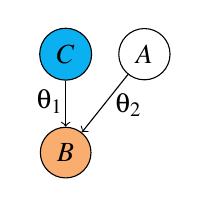
\begin{tikzpicture}
  \node (s0) at (0,1.25) [circle,draw=black,fill=ProcessBlue] {$C$};
  
  \node (s2) at (0,0) [circle,draw=black,fill=Apricot] {$B$};
  
  \node (s3) at (1,1.25) [circle,draw=black] {$A$};
 
  \path (s0) edge[->] (s2);
  
  \path (s3) edge[->] (s2);
  
  \node (l1) at (-.2,.65) {$\theta_1$};
  
  \node (l1) at (.8,.6) {$\theta_2$};
  
 \end{tikzpicture}
\hspace{.7in}
  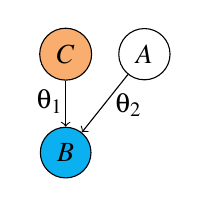
\begin{tikzpicture}
  
  \node (s0) at (0,1.25) [circle,draw=black,fill=Apricot] {$C$};
  
  \node (s2) at (0,0) [circle,draw=black,fill=ProcessBlue] {$B$};
  
  \node (s3) at (1,1.25) [circle,draw=black] {$A$};
 
  \path (s0) edge[->] (s2);
  
  \path (s3) edge[->] (s2);
  
    \node (l1) at (-.2,.65) {$\theta_1$};
  
  \node (l1) at (.8,.6) {$\theta_2$};
  
 \end{tikzpicture} \end{center}
 \caption{Predictive versus Diagnostic Inference} \label{diagnostic}
\end{figure}
The left diagram depicts a predictive inference, where effect $B$ is queried given evidence that cause $C$ is active. On the right is a diagnostic inference, where the causal variable $C$ is queried given evidence $B$. In this simple model, we can fold $P(A)$ and $\theta_{B,A}$ into a single parameter $\theta_2$, so that $A$ effectively has prior probability 1, and the resulting conditional probabilities can be simplified to: 
$$P(B\mid C) \;= \; \theta_1 + \theta_2 - \theta_1\theta_2$$
$$P(C \mid B) \;= \; 1- \big(1-P(C)\big)\Big(\theta_2\;/\;\big(P(C)\theta_1 + \theta_2  - P(C)\big)\Big)$$
The finding in \cite{Fernbach2011} is that subjects routinely ignore variable $A$ in predictive inference tasks, and thereby consistently make low estimates of $P(B\mid C)$. In diagnostic inference tasks, however, subjects show sensitivity to strength and number of alternatives, consequently making more accurate judgments. Indeed, there is a longer reaction time for diagnostic than for predictive inferences, and only in the diagnostic condition is there dependency of reaction time on number of alternatives \citep{Fernbach2010}. \cite{Fernbach2013} verified that this asymmetry between diagnostic and predictive reasoning is robust; in particular, it not due to availability or memory limitations.

In other words, subjects seem to be reasoning with a submodel, ignoring variable $A$, in the predictive case, but not in the diagnostic case. How detrimental could it be to neglect $A$ for these two types of inference. Again, consider first KL-divergence. Without a background bias term (as in the previous example), for the diagnostic case ignoring variable $A$ will lead to the conclusion that $C$ has probability 1, which means the KL-divergence is not even defined. With a positive bias term, we can make the KL-divergence as large as we like, by making the bias smaller. For instance, with $\beta = 0.01$, the average value of $KL(P\;||\;P^*)$ is already $1.740$, extremely high, in the diagnostic case. By contrast, it is only $0.298$ in the predictive case. Assuming general accuracy matters, it would seem reasonable, at least on average, to neglect variables in the predictive rather than the diagnostic cases.

How does this look from the perspective of expected utility, again assuming a single-sample-based agent?  Table \ref{predictive} shows the differences in expected utility for several parameter settings between the EU of using the true distribution and the approximate distribution (ignoring variable $A$), for both the predictive and diagnostic cases. 
\begin{table}[h]  \begin{center}
\begin{tabular}{c | c | c || c | c}
 $P(C)$ & $\theta_1$ & $\theta_2$ & $\Delta_{pred}$ & $\Delta_{diag}$ \\ \hline
  $0.1$ & $0.3$ & $0.9$ & $1.083$ & $1.345$ \\
 $0.5$ & $0.9$ &  $0.9$ & $0.176$ & $-0.041$ \\
 $0.5$ & $0.5$ & $0.1$ & $0.010$ & $-0.144$ \\
  $0.2$ & $0.3$ & $0.2$ & $-0.034$ & $0.345$ \\
 $0.1$ & $0.3$ & $0.1$ & $-0.036$ & $0.550$ \\

\end{tabular} \end{center} \caption{Differences in expected utility between the true and approximate distributions, for predictive and diagnostic inferences (with $\beta = 0.05$ for diagnostic cases).} \label{predictive}
\end{table} 
In some cases, $\Delta_{pred}$ is indeed smaller than $\Delta_{pred}$, meaning that the agent suffers less in expected utility when using the smaller submodel. However, there are also cases where $\Delta_{pred}$ is quite large, e.g., $\approx 0.1$, even when $\Delta_{diag}$ is small. Indeed, the average $\Delta_{pred}$ value, over $0.01$ intervals for all parameters, is $0.198$---quite large, and significantly greater than $\Delta_{diag}$, whose average is $0.044$. Moreover, \cite{Fernbach2013} have shown that people exhibit neglect even in these cases where the mistake is rather serious. Thus, if we consider the single-sampling agent, and average over all parameter settings, it would seem that people ignore alternatives in the \emph{altogether wrong} cases.


If we take resource rationality as a working methodological hypothesis, this would suggest at least two conclusions. First, in simple situations like in Figure \ref{diagnostic}, people may not make decisions based on a single sample, which is after all a strategy that makes more sense in computationally demanding tasks---they may either take more samples, or use a different algorithmic strategy altogether. Relatedly, people may often face decision problems that call for more fine-grained judgments: not just which outcome is more likely, but how much more likely. For such tasks, KL-divergence matters.

Second, the results of \cite{Fernbach2011}, together with the proposed analysis, strongly suggest that people may optimize grain of representation only at a high level of abstraction, in terms of general features such as the type of inference in question (predictive versus diagnostic). Understanding how this might work will require expanding the analysis, e.g., to incorporate elements of metalevel control \citep{Icard2014,Lieder2014}, and further experimental work to understand under what conditions, and to what extent, alternatives are ignored.

\section{Further Questions and Directions}

%NDG: point out that this leaves open the problem of optimizing the params in the moment....

Dynamic view: Could consider a probabilistic generalization of the ``contradiction hypothesis" of Park \& Sloman (2013), concerning when to ``add'' a new causal variable. \cite{KlaymanHa}: people go with a hypothesis until it is contradicted by data. Confirmation only adds to it.

Previous work on ``relevance'' of variables in graphical models \citep{Druzdzel}

More general class of approximation strategies: combining with MCMC strategies, etc. \citep{WickMcCallum}

``The frame problem goes very deep; it goes as deep as the analysis of rationality" \citep{Fodor1987}

%NDG: should do joint optimization of samples and submodel.
%TFI: Yes!

\bibliographystyle{apalike}

\bibliography{bayes}


\end{document}
